\documentclass[a4paper,11pt]{article}
\usepackage{latexsym}
\usepackage{hyperref}
\usepackage{graphicx}
\usepackage[MeX]{polski}
\usepackage[utf8]{inputenc}
\author{Adam Gonstal	Kamil Kolasa	Rafał Kornel	Konrad Maliszewski	Anna Olechowska}
\title{Poszukiwanie mikrosoczewek grawitacyjnych}
\frenchspacing
\newcommand{\ak}{\hspace{1.0cm}}
\begin{document}
\maketitle
\newpage
\tableofcontents
\newpage
\section{Abstrakt}
\ak Poniżej opisany projekt studencki polegał na analizie fragmentu danych z projektu OGLE III w celu znalezienia zjawisk mikrosoczewkowania grawitacyjnego.  Autorom zostały udostępnione dane z teleskopu w Las Campanas w Chile, dotyczące m.in. pomiarów jasności dla ok. $260$ tysięcy  gwiazd, zbieranych na przestrzeni ok. $6$ lat. W ramach projektu utworzony został algorytm analizujący dane dla każdej gwiazdy i zwracający wykresy zależności jasności od czasu dla tych gwiazd, które według algorytmu mogły dawać efekt soczewki. Około $x\%$ zwróconych gwiazd okazało się rzeczywistymi przypadkami mikrosoczewkowania grawitacyjnego. Ponadto, $y$ ze znalezionych przez algorytm soczewek nie zostały zidentyfikowane przez zespół projektu OGLE III.
\section{Wstęp}
\subsection{Wstęp teoretyczny}
\ak Zjawisko soczewkowania grawitacyjnego wynika z zakrzywienia czasoprzestrzeni przez masy znajdujące się w niej. Konsekwencją tego jest poruszanie się promieni świetlnych po zakrzywionych torach, tj. najkrótszych możliwych, ale w przestrzeni Mińkowskiego. W związku z tym, w sytuacji gdy w okolicach linii łączącej źródło światła (np. galaktykę) z obserwatorem znajdzie się odpowiednio duża masa, światło biegnie omijając taką masę, co przedstawia Rysunek \ref{Fig_1}. 

\begin{figure}[h]
\centering
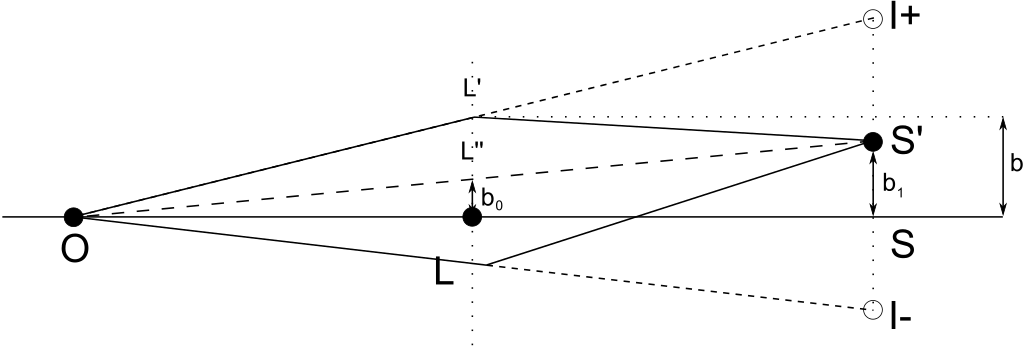
\includegraphics[width=0.9\textwidth]{Fig/Lens.jpeg}
\label{Fig_1}
\caption{Przykład zjawiska soczewkowania, gdzie źródło S' jest obserwowane jako dwa obrazy I+ i I-\cite{Lens}.}
\end{figure}

\ak Obraz źródła widziany przez obserwatora może ulec różnym deformacjom, tj. rozciągnięciu, przemieszczeniu, kilkukrotnemu odbiciu, a także wzmocnieniu, co w przypadku tego projektu jest najistotniejszym aspektem soczewkowania. Przykłady takiego zjawiska przedstawiają Rysunki \ref{Fig_2} i \ref{Fig_3}.
\newpage%UWAGA NEWPAGE
\begin{figure}[h]
\centering
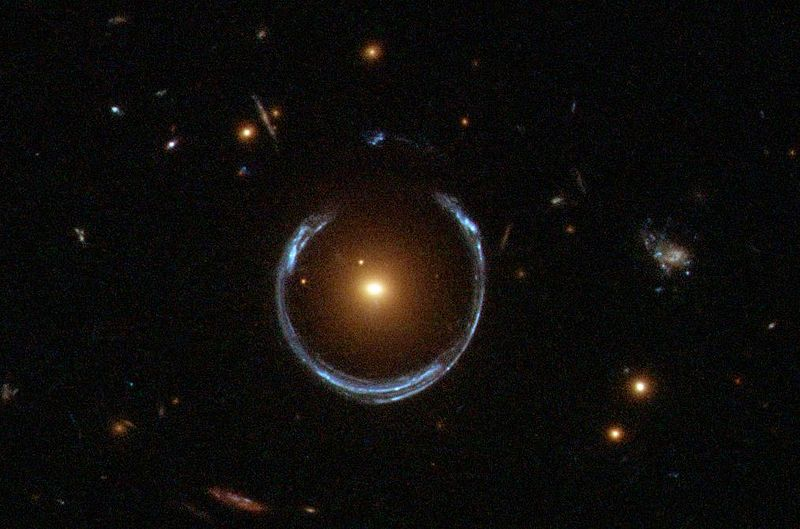
\includegraphics[width=0.4\textwidth]{Fig/Horseshoe.jpeg}\hspace{1.7cm}
\label{Fig_2}
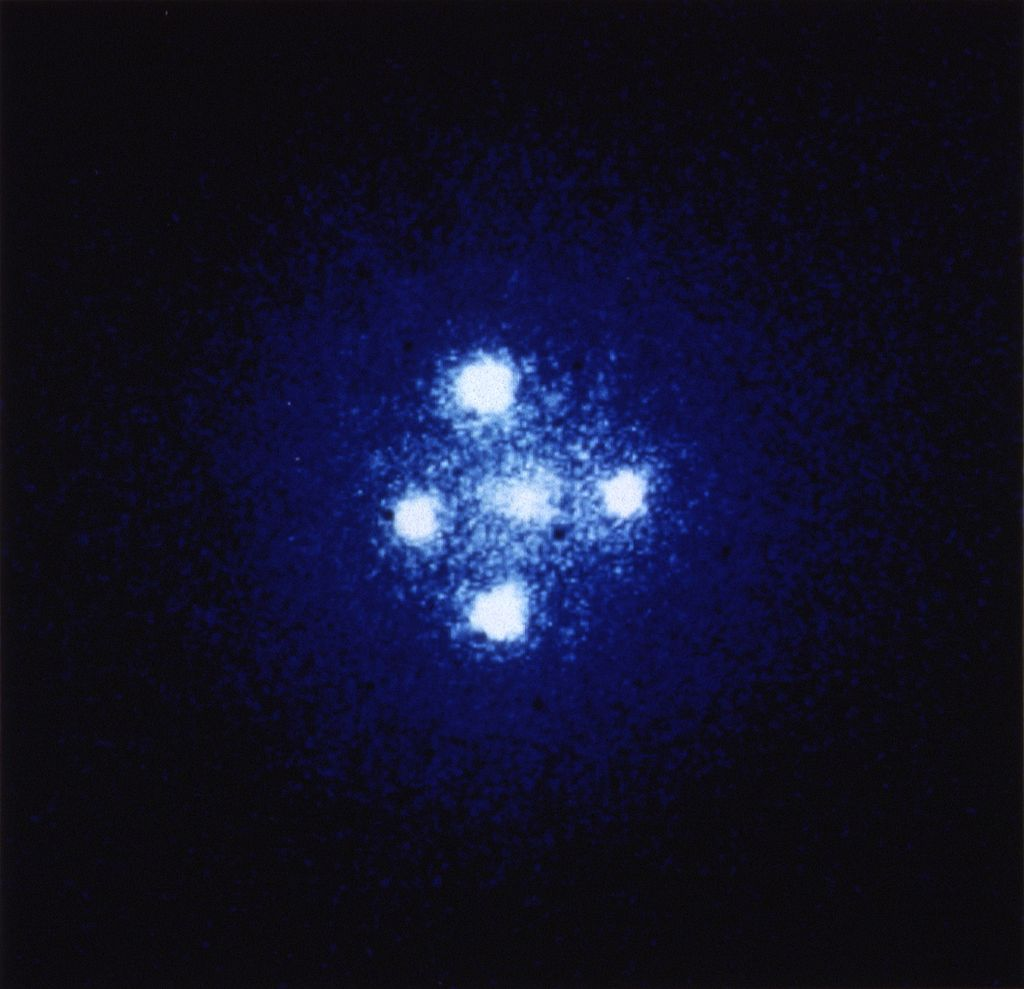
\includegraphics[width=0.3\textwidth]{Fig/Cross.jpeg}
\label{Fig_3}
\end{figure}
\begin{table}[h]
\begin{tabular}{cc}
\begin{tabular}[c]{@{}c@{}}Rysunek 2.1: Galaktyka LRG 3-757 \\ soczewkująca obraz galaktyki \\ znajdującej się za nią\cite{Horseshoe}.\end{tabular} & \begin{tabular}[c]{@{}c@{}}Rysunek 2.2: Kwazar Q2237+030 \\ soczewkowany przez galaktykę \\ ZW 2237+030, tzw. krzyż Einsteina\cite{Cross}.\end{tabular}
\end{tabular}
\end{table}

\ak W szczególnych przypadkach, gdy masa soczewkująca jest stosunkowo nieduża, a jej tor ruchu przecina bądź jest bardzo bliski torowi promieni świetlnych od źródła do obserwatora, efekty deformacji obrazu mają zbyt małe rozmiary kątowe, by udało się je zaobserwować z Ziemi. W takich sytuacjach jedyną obserwowalną konsekwencją zajścia soczewki jest wzmocnienie jasności. Ten specyficzny rodzaj soczewkowania nazywany jest mikrosoczewkowaniem grawitacyjnym. Przykładem jego może być obiekt z pobliskiej galaktyki wysyłający ku Ziemi promieniowanie elektromagnetyczne, na którego drodze znajduje się masywna planeta. Wzmocnienie można wyrazić jako wielkość $\mu$, będącą ilorazem strumienia światła bez wzmocnienia oraz z wzmocnieniem. Ponieważ natężenie światła $I$ jest stałe w czasie, będzie to wyłącznie iloraz kątów bryłowych, z których światło dociera do  obserwatora.\\
\begin{equation}
\centering
\mu=\frac{Id\Omega}{Id\Omega_{0}}=\frac{d\Omega}{d\Omega_{0}}
\label{Eq_1}
\end{equation}
\flushleft
\ak Wzmocnienie można również dobrze opisać za pomocą odległości $u$ źródła światła od soczewki, którą można opisać za pomocą kilku parametrów, które dla danej soczewki można przyjąć jako stałe w trakcie trwania zjawiska. Wspomniane parametry gemetryczne mają wpływ na $t_{E}$, tj. czas Einsteina. Wielkość $b$ jest wielkością analogiczną do parametru zderzenia i także jest stała. Czas $t_{0}$ jest momentem największego wzmocnienia, z kolei jedyną zmienną we wzorze \ref{Eq_2} jest czas {t}.
\begin{equation}
\centering
u(t)=\sqrt{\left(\frac{t-t_{0}}{t_{E}}\right)^{2}+b^{2}}
\label{Eq_2}
\end{equation}
\ak Znając już zależność $u(t)$ można powiązać ją ze wspomnianym wcześniej wzmocnieniem $\mu$, tj. wyprowadzić wzór \ref{Eq_3}, zwany także krzywą Paczyńskiego. Przykładową krzywą Paczyńskiego przedstawia Rysunek \ref{Fig_997}. %tutaj ref do krzywej w subsection "Projekt OGLE"
W skali sześciu lat mikrosoczewka trwająca ok. $70$ dni widocznie wyróżnia się skokiem jasności w trakcie trwania zjawiska, co było punktem wyjściowym przy konstrukcji algorytmu i zostanie opisane dokładniej w kolejnych rozdziałach.
\begin{equation}
\centering
\mu(u)=\frac{u^{2}+2}{u\sqrt{u^{2}+4}}
\label{Eq_3}
\end{equation}
\flushleft
\subsection{Projekt OGLE}

\section{Analiza danych}

\section{Rezultaty}

\section{Bibliografia}
\begin{thebibliography}{99}
\bibitem{Lens} \url{https://pl.wikipedia.org/wiki/Soczewkowanie_grawitacyjne#/media/Plik:Dwa_promienie.svg}
\bibitem{Horseshoe} \url{https://en.wikipedia.org/wiki/File:A_Horseshoe_Einstein_Ring_from_Hubble.JPG}
\bibitem{Cross} \url{https://pl.wikipedia.org/wiki/Krzy%C5%BC_Einsteina#/media/Plik:Einstein_cross.jpg}
\end{thebibliography}
\end{document}
